%%%%%%%%%%%%%%%%%%%% Documentación del usuario %%%%%%%%%%%%%%%%%%%%

\section{Documentación de usuario}

\subsection{Descripción funcional}

Este programa ha sido creado con la finalidad de brindar un servicio de compartición de coches a los miembros de la comunidad universitaria de la Escuela Superior de Ingeniería. 
Con esto, se conseguirá una gran reducción de los costes diarios de transportes, al igual que una significante disminución de gases.

\bigskip

Como hemos comentado anteriormente, queremos dar un servicio de calidad, es por esto que con nuestro programa usted podrá realizar diferentes acciones, como:
\begin{itemize}
  \item Siendo \textbf{Pasajero} se le permitirá:
  \begin{itemize}
    \item Consultar y variar sus datos personales.
    \begin{center}
      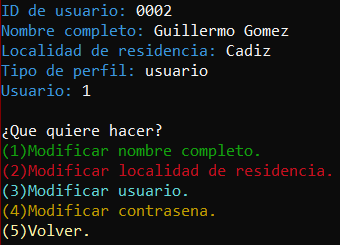
\includegraphics[]{FOTOS/menuPasajeroPerfil.png}
    \end{center}
    \newpage
    \item Reservar y cancelar viajes.
    \begin{center}
      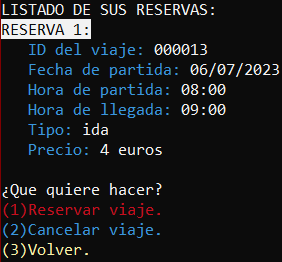
\includegraphics[]{FOTOS/menuPasajeroViaje.png}
    \end{center}
  \end{itemize}
  \item Siendo \textbf{Conductor} se le permitirá:
  \begin{itemize}
    \item Consultar y cambiar sus datos personales.
    \begin{center}
      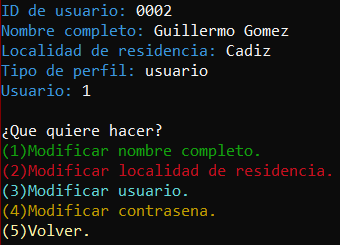
\includegraphics[]{FOTOS/menuPasajeroPerfil.png}
    \end{center}
    \newpage
    \item Dar de alta, modificar y eliminar vehículos.
    \begin{center}
      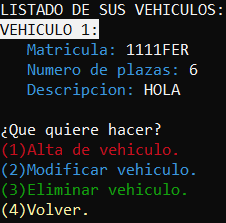
\includegraphics[]{FOTOS/menuConductorVehiculo.png}
    \end{center}
    \item Crear, modificar, anular y finalizar viajes.
    \begin{center}
      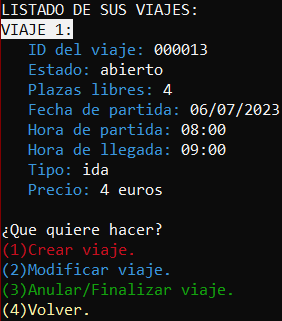
\includegraphics[]{FOTOS/menuConductorViaje.png}
    \end{center}
  \end{itemize}
  \newpage
  \item Siendo \textbf{Administrador} se le permitirá:
  \begin{itemize}
    \item Crear, descartar, cambiar y listar usuarios.
    \begin{center}
      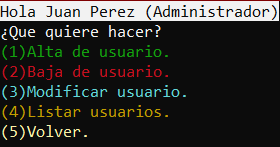
\includegraphics[]{FOTOS/menuAdminUsuario.png}
    \end{center}
    \item Dar de alta, suprimir, variar y listar vehículos.
    \begin{center}
      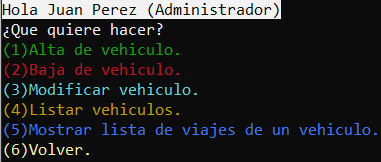
\includegraphics[]{FOTOS/menuAdminVehiculo.png}
    \end{center}
    \item Establecer, anular, finalizar, cancelar, modificar y listar viajes.
    \begin{center}
      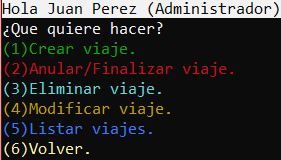
\includegraphics[]{FOTOS/menuAdminViaje.png}
    \end{center}
  \end{itemize}
\end{itemize}

\newpage

\subsection{Limitaciones}

El proyecto tiene algunas restricciones, las cuales han sido impuestas para que no haya fallos, aunque esto ha hecho que hagan falta más líneas de código.
\begin{itemize}
  \item En todos los escaneos, se tiene que introducir como mínimo 1 dígito/carácter.
  \item Dos usuarios no pueden tener el mismo nombre de usuario en la base de datos.
  \item Se ha realizado una lista con las siglas de todas las localidades de la provincia de Cádiz, para evitar errores a la hora de comparar las ciudades.
  \item Al introducir una fecha y horas, tienen que ser posteriores a las actuales, el año introducido debe ser posterior a 2022.
  \item Para darle de alta a un vehículo, su matrícula tiene que ser correcta (con 4 dígitos y 3 caracteres) y no puede estar registrada en el sistema. Además, el número de plazas debe estar entre 1 y 9.
  \item No se puede ni modificar ni eliminar un vehículo, si tiene viajes abiertos, con plazas ocupadas, o iniciados o cerrados.
  \item Sólo se pueden modificar o anular viajes, si no tienen ninguna plaza ocupada.
  \item No se puede tener más de 1 viaje abierto con un vehículo en un mismo día, es decir, si quieres crear un viaje para esa fecha, primero debes acabar el que ya esté abierto.
  \item Para finalizar un viaje, este debe estar iniciado.
\end{itemize}
\label{fig:Limitaciones}

\subsection{Tecnología}

Este programa lo hemos realizado con el entorno de desarrollo integrado (IDE) \href{https://www.codeblocks.org/}{Code::Blocks}, en su versión 20.03.
A la hora de programar, hemos tenido que emplear diferentes bibliotecas, como:
\begin{itemize}
  \item stdio.h: Manejar la entrada y salida de datos a través de archivos, dispositivos de entrada/salida estándar, etc.
  \item string.h: Usar cadenas de caracteres.
  \item stdlib.h: Emplear estructuras, memoria dinámica, conversión de cadenas, etc.
  \item locale.h: Proporcionar el uso de caracteres especiales de un idioma.
  \item windows.h: Incluir comandos del sistema operativo Microsoft Windows.
  \item conio.h: Utilizar la entrada y salida de caracteres por la consola.
  \item time.h: Trabajar con fechas y tiempos.
\end{itemize}

\bigskip

Por ejemplo, se han empleado vectores con estructuras dinámicas, o incluso matrices/vector de vectores dinámicos, esto se puede observar en el módulo Buscar \ref{fig:BuscarCod},
hemos usado memoria dinámica en gran parte del proyecto, para reducir la carga del mismo, y hacer que todo tipo de ordenadores puedan ejecutarlo. 
Además, hemos utilizado la función atoi, para hacer que no se tenga que introducir la ID del usuario entera, por ejemplo, "0004", con poner "4", ya funciona.
También se ha hecho uso de ficheros temporales, para eliminar/modificar, como se puede ver en en los módulos Eliminar \ref{fig:EliminarCod} y Modificar \ref{fig:ModificarCod}.

\subsection{Manual de instalación}

Para usar el programa, sólo tiene que dirigirse a la carpeta \href{run:./../../SETUP}{SETUP}, donde encontrará un acceso directo, llamado ESI-SHARE, que tiene como ruta, el archivo ejecutable del programa.
Otra forma sería instalar \href{https://www.codeblocks.org/}{Code::Blocks}, y ejecutar el archivo de proyecto ESI-SHARE.cbp.
\newpage
\begin{itemize}
  \item Requisitos mínimos del sistema:
  \begin{itemize}
    \item Procesador: Intel Core i3 ó AMD Athlon II
    \item Memoria RAM: 2GB
    \item Espacio en disco duro: 100MB
  \end{itemize}
  \item Es recomendable usar cualquier versión de Windows, para que no haya conflicto a la hora de usar algunas funciones.
\end{itemize}

\bigskip

\subsection{Acceso al sistema}

Tras haber iniciado el programa, se encontrará un menú, en el que encontrará dos opciones, una para acceder al sistema, si ya tiene unas credenciales, y otra para registrarse,
que le pedirá sus datos personales, para darse de alta. Si quiere testear el acceso al sistema, puede introducir:
\begin{itemize}
  \item Para acceder como usuario:
  \begin{itemize}
    \item Usuario: \textbf{usua1}
    \item Contraseña: \textbf{2023}
  \end{itemize}
  \item Para acceder como administrador:
  \begin{itemize}
    \item Usuario: \textbf{admin}
    \item Contraseña: \textbf{1234}
  \end{itemize}
\end{itemize}

A la hora de salir, se ha elaborado un mecanismo intuitivo y sencillo, ya que en todo momento podrá volver al menú anterior, introduciendo el número indicado por pantalla.
En el caso de querer salir totalmente del programa, tendrá que cerrar sesión, volviendo al menú principal.
\begin{center}
  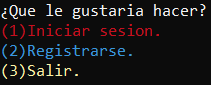
\includegraphics[]{FOTOS/menuPrincipal.png}
  \label{fig:menuPrincipal}
\end{center}

\subsection{Manual de referencia}

El programa le puede aportar un gran ahorro de dinero en desplazamientos, debido al óptimo sistema de reservas que desempeña, haciendo posible que cualquier estudiante, profesor o personal
de la Escuela Superior de Ingeniería, pueda acceder a dichas ventajas.

\bigskip

Cuando ejecute al programa, podrá acceder con sus credenciales, o registrarse. Si accede con sus credenciales, tendrá las opciones de ser "Pasajero" ó "Conductor", 
dependiendo de lo que quiera hacer, seleccionará uno u otro, esto se puede cambiar en cualquier momento, volviendo a dicho menú. \ref{fig:menuPrincipal}

\begin{itemize}
  \item Si elige la opción de ser \textbf{Pasajero}, podrá:
  \begin{itemize}
    \item Entrar en el menú de \textbf{Perfil}, donde puede ver todos sus datos personales, al igual que si selecciona una de las opciones, podrá modificar cada uno de sus datos.
    \item Acceder al menú de \textbf{Viajes}, en el que se le permitirá reservar un viaje ya existente que pase por su localidad, al igual que cancelar cualquier reserva.
  \end{itemize}
  \item Si elige la opción de ser \textbf{Conductor}, podrá:
  \begin{itemize}
    \item Entrar en el menú de \textbf{Perfil}, donde puede ver todos sus datos personales, al igual que si selecciona una de las opciones, podrá modificar cada uno de sus datos.
    \item Pasar al menú de \textbf{Vehículos}, para introducir nuevos vehículos, modificarlos o incluso eliminarlos. Para esto, la matrícula del vehículo no puede existir en la base de datos.
    \item Acceder al menú de \textbf{Viajes}, en el que se le permitirá crear un viaje nuevo, siempre y cuando no haya dos abiertos en el mismo día, habría que acabar uno para empezar el siguiente,
    todo esto con el objetivo de que no se solapen los viajes. Además, se pueden modificar los viajes, si estos están abiertos y sin plazas reservadas, e incluso anular ó finalizar los viajes,
    esta selección la hará automáticamente el sistema, dependiendo del estado del viaje.
  \end{itemize}
\end{itemize}

Asimismo, hay un menú especial, si accede con las credenciales del \textbf{Administrador}. En este menú, tendrá acceso a todo tipo de información de la base de datos, como:
\begin{itemize}
  \item Entrar en el menú de \textbf{Usuarios}, donde puede crear un usuario desde cero, eliminar cualquier usuario del sistema, modificar los datos personales de cualquiera,
  e incluso obtener una lista con todos los usuarios que hay en el sistema.
  \item Pasar al menú de \textbf{Vehículos}, para dar de alta nuevos vehículos, eliminar un vehículo, modificar los datos de un vehículo, imprimir una lista de todos los vehículos que hay registrados
  al igual que obtener el historial de todos los viajes que ha realizado un vehículo, a partir de su matrícula.
  \item Acceder al menú de \textbf{Viajes}, en el que se le permitirá registrar un viaje, anular/finalizar, eliminar y modificar cualquier viaje del sistema, y obtener una lista con todos los viajes
  que hay registrados en el sistema.
\end{itemize}